% \cite{3288} gibt eine Einführung zu \textit{Dithering mit blue noise}. Darunter ist ein abbilden
% beliebiger Grauwerte zu einer Menge von blue noise verteilten Schwarz- und Weißwerten zu verstehen.
Eine Ansammlung von Pixeln, deren Verteilung über den Raum einer blue noise entspricht, 
weist eine Reihe von Eigenschaften

\begin{itemize}

    \item \nameref{ch:Content1:sec:blue noise:Uniformität}
    \item \nameref{ch:Content1:sec:blue noise:Isotropie}
    \item \nameref{ch:Content1:sec:blue noise:Kachelung}
    \item \nameref{ch:Content1:sec:blue noise:Niedrige Frequenzen}

\end{itemize}

zur Steigerung der visuellen Qualität des Bildes auf. \cite{3288}
Im Folgenden wollen wir uns diese Eigenschaften genauer anschauen.
Hierfür verwenden wir die in \cite{Pet17} vorgestellten Texturen, welche anhand der
\textit{Void and Cluster}-Methode(siehe \cite{ulichney1993void}) erstellt wurden.

\subsection{Eigenschaften}

Um die Eigenschaften der Texturen zu untersuchen wurden korrespondierende Spektren zu den Texturen mit Hilfe von 
\cite{JCrystalSoft2018} erstellt und miteingebunden.

\subsubsection{Uniformität}
\label{ch:Content1:sec:blue noise:Uniformität}

Für die Wahrscheinlichkeitsfunktion, dass
ein Pixel mit Grauwert p bei der Generierung ausgeben wird  ($\textit{p} \in [0,1]$) muss gelten: 

\begin{equation}\label{eq:Uniformitätsgleichung}
    P(n \leq p) = p
\end{equation}

Die Uniformität(lat. \textit{uniformitas}-Einförmigkeit) garantiert uns dieses
Verhalten $\forall p \in [0,1]$. Man könnte auch sagen, dass jeder Grauwert gleichwahrscheinlich
auftreten soll. Die zugehörige konstante Wahrscheinlichkeitsdichte
lässt sich einfach zur Echtzeit umsetzen mit Hilfe von (pseudo-)zufälligen Zahlen.
Mit der erstellten(siehe Werkezug \cite{WhiteNoiseGenerator}) white noise Textur,

\label{pic:white noise}
\begin{figure}[H]
    \centering
    \begin{minipage}[t]{0.45\linewidth}
        \centering
        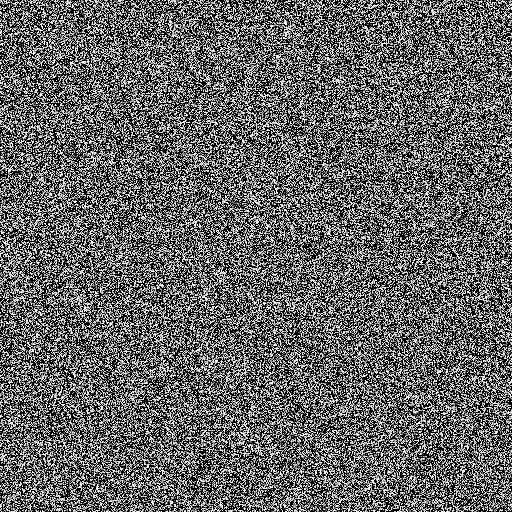
\includegraphics[width=\linewidth]{content/BlueNoise/Bilder/whitenoise.png}
        \caption{white noise Textur}
    \end{minipage}
    \hfill
    \begin{minipage}[t]{0.45\linewidth}
        \centering
        
\includegraphics[width=\linewidth]{content/BlueNoise/Bilder/FFT_whitenoise.png}
        \caption{Amplitudenspektrum}
        \label{pic:FrequenzspektrumWhiteNoise}
    \end{minipage}
\end{figure}

ergibt sich eine typische Amplitudendichte. Zufällig verteilt, über alle 
Frequenzen hinweg. Mit diesem weißen Rauschen arbeitet man klassischerweise in einem \nameref{ch:Content1:sec:Path Tracer}.
Diese Uniformität garantiert dabei die Unkorreliertheit der Pixelfolgen. Wir merken also, dass 
diese Eigenschaft alleine nicht ausreicht und uns zur Eigenschaft der niedrigen Frequenz führt.

\subsubsection{Niedrige Frequenzen}
\label{ch:Content1:sec:blue noise:Niedrige Frequenzen}
Niedrige Frequenzen sind in einer blue noise sehr wenig bis gar nicht 
vertreten. Dies macht sich sowohl in der Zeitdomäne erkenntlich: keine erkenntlichen gleichfarbigen Pixelverbünde 
innerhalb der Textur als auch in der Frequenzdomäne: der schwarze Ring innerhalb der Amplitudendichte
deutet auf das Fehlen von niederen Frequenzen und dem hohen Unterschied benachbarter Pixel hin.
Außerdem haben wir aus der vorherigen Eigenschaft der \nameref{ch:Content1:sec:blue noise:Uniformität} gesehen:
Wir wollen das alle Grauwerte gleichwahrscheinlich auftreten. Dies können wir am besten im Frequenzspektrum 
(siehe \ref{pic:FrequenzspektrumBlueNoise})
beobachten. Hier sind alle hohen Frequenzen wie beim weißen Rauschen \ref{pic:FrequenzspektrumWhiteNoise} gleich stark vertreten.

\label{pic:blue noise}
\begin{figure}[H]
    \centering
    \begin{minipage}[t]{0.45\linewidth}
        \centering
        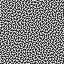
\includegraphics[width=\linewidth]{content/BlueNoise/Bilder/HDR_L_0.png}
        \caption{$512^{2}$ blue noise Textur}
    \end{minipage}
    \hfill
    \begin{minipage}[t]{0.45\linewidth}
        \centering
        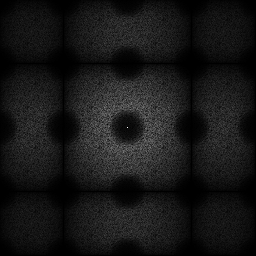
\includegraphics[width=\linewidth]{content/BlueNoise/Bilder/FFT_HDR_L_0.png}
        \caption{Fourier Spektrum $512^{2}$ blue noise Textur}
        \label{pic:FrequenzspektrumBlueNoise}
    \end{minipage}
\end{figure}

Auch zu erkennen ist die weitere Eigenschaft der \nameref{ch:Content1:sec:blue noise:Isotropie}.

\subsubsection{Isotropie}
\label{ch:Content1:sec:blue noise:Isotropie}

Die Isotropie(altgr. \textit{isos}-gleich und \textit{tropos}-Richtung)
einer blue noise Textur bietet eine weitere wichtige Eigenschaft. Dabei haben wir in allen Dimensionen
die Unabhängigkeit einer Eigenschaft. Um uns dies an einem Gegenbeispiel 
klar zu machen, schauen wir uns das Bayer-Pattern an. Dieses Pattern erfüllt sowohl 
die Eigenschaft der Niedrigen Frequenz (siehe Abschnitt \ref{ch:Content1:sec:blue noise:Niedrige Frequenzen}) als auch 
die der \nameref{ch:Content1:sec:blue noise:Uniformität}, jedoch nicht Jene der Isotropie.
Zu erkennen ist dies an den sich wiederholenden Strukturen in der Abbildung \ref{pic:bayer pattern}.

\label{pic:bayer pattern}
\begin{figure}[H]
    \centering
    \begin{minipage}[t]{0.45\linewidth}
        \centering
        
\includegraphics[width=\linewidth]{content/BlueNoise/Bilder/BayerMatrix.png}
        \caption{$512^{2}$ bayer pattern Textur}
    \end{minipage}
    \hfill
    \begin{minipage}[t]{0.45\linewidth}
        \centering
        
\includegraphics[width=\linewidth]{content/BlueNoise/Bilder/FFT_BayerMatrix.png}
        \caption{Amplitudendichte $512^{2}$ bayer pattern Textur}
        \label{pic:Frequnzdomäne Bayer}
    \end{minipage}
\end{figure}

In der Frequenzdomäne (Abbildung \ref{pic:Frequnzdomäne Bayer}) ist zu erkennen, dass die Amplitudendichte in einzelnen
Punkten organisiert ist. Diese lassen sich durch die vorhandenen
Richtungen der Textur erklären. Speziell in zwei Richtungen ist eine sich
wiederholende Pixelsequenz zu erkennen.
Allerdings wollen wir in alle Richtungen eine gleiche (isotrope!) 
Verteilung.

\subsubsection{Kachelung}
\label{ch:Content1:sec:blue noise:Kachelung}

Im Gegensatz zu dem bayer pattern oder der white noise, die sich einfach zur Echtzeit berechnen lassen,
sind blue noise verteilte Texturen im Erstellungsaufwand, der mit Anzahl der Dimensionen 
und Größe der Textur schnell anwächst, deutlich höher (siehe auch \cite{bluenoisechrisschied}). 
Es empfiehlt sich daher für den temporalen Algorithmus in Kapitel \ref{ch:Temporaler Algorithmus} eine 
kleinere Textur zu verwenden.
Dies hat außerdem den Vorteil, eine bessere Ausnutzung des kleinen aber schnellen Cachespeichers zu gewährleisten.
Aufgrund des Aufbaus von aktueller Grafikhardware (siehe \cite{turingarchitecture}) wollen wir diese Textur
soweit oben wie möglich in der Cachehierarchie halten.(L1 96KByte, L2 6MByte).

\label{pic:tiled blue noise}
\begin{figure}[H]
    \centering
    \begin{minipage}[t]{0.45\linewidth}
        \centering
        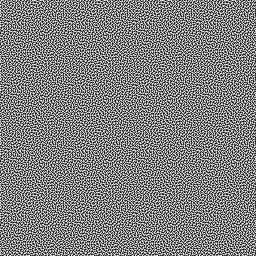
\includegraphics[width=\linewidth]{content/BlueNoise/Bilder/tiled4times.png}
        \caption{$512^{2}$ gekachelte Textur von $64^{2}$}
    \end{minipage}
    \hfill
    \begin{minipage}[t]{0.45\linewidth}
        \centering
        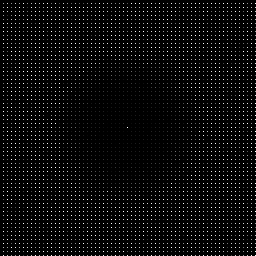
\includegraphics[width=\linewidth]{content/BlueNoise/Bilder/FFTtiled4times.png}
        \caption{Fourier Spektrum}
    \end{minipage}
\end{figure}

Betrachtet man die Abbildung \ref{pic:tiled blue noise} lässt sich der blue noise Charakter anhand des
wenigen niederen Frequenzanteils erkennen. Wiederholungen sind in der Zeitdomäne schwerer zu erkennen. 
Obwohl Sie in der Frequenzdomäne erkennbar sind und unsere \nameref{ch:Content1:sec:blue noise:Isotropie}
(teilweise) aufheben. Um dieses Problem zu umgehen werden wir mit Hilfe von \nameref{ch:Content1:sec:Quasi-Zufallsfolgen}
auf diese Textur zugreifen und die Isotropie (teilweise) wiederherstellen.
Daher können wir hier folgendes Fazit ziehen: Regelmäßige Kachelung einer kleineren \nameref{ch:Content1:sec:blue noise} Textur 
über das gesamte Bild liefert eine gute \nameref{ch:Content1:sec:blue noise} Verteilung bei vertretbaren Rechenaufwand und guter 
Cacheausnutzung!\cite{turingarchitecture}
\todo{explain cachausnutzung}

%% ===========================
\section{Dithering Sampling}
\label{ch:Content1:sec:blue noise sampling}
\label{subsec:dither sampling}
Nachdem wir die Eigenschaften der \nameref{ch:Content1:sec:blue noise} kennengelernt haben,
können wir zusammen mit dem Verständnis über den \nameref{ch:Content1:sec:Path Tracer} und der 
zugrundeliegenden Monte-Carlo Integration (siehe Gleichung \ref{eq:Monte-Carlo}) das \glqq dithered sampling\grqq{} verstehen.
\textit{Dithering} ist das bewusste Einbringen eines Rauschens, um entstehende Quantisierungsfehler zu randomisieren.
Klassischerweise wird eine zweidimensionale \nameref{ch:Content1:sec:blue noise} Textur verwendet, um mit einer darauf aufbauenden Schwellenwertbildung,
dieses Rauschen in ein Bild zu bringen. Hier wollen wir durch Dithering die Verteilung des entstehenden Monte-Carlo Integrationsfehlers (Rauschen) verändern.\par
Grundlage des n-dimensionalen Path Tracers werden sowohl eine \nameref{ch:Content1:sec:blue noise}-Verteilung als auch Anfangswerte $s_{n}$ mit d-Dimensionen.
Damit konkretisiert sich die Monte-Carlo Integration (siehe Gleichung \ref{eq:Monte-Carlo}) mit Integrand f zu folgender Gleichung:

\begin{tcolorbox}[rightrule=3mm, rounded corners=east]
    \begin{equation}\label{eq:concreteMonteCarlo}
        \frac{1}{N}\sum_{n=0}^{N-1}f(s_{n})
    \end{equation}
\end{tcolorbox}


Mit dem Ziel, eine blue noise Fehlerverteilung im Bildraum zu erreichen, hat sich bereits die Arbeit \cite{georgiev2016blue} beschäftigt. 
Mit im Vorraus (\glqq a priori\grqq{}) blue noise korrelierten Zahlenfolgen $s_{n}$ hoffte man ebenso korrelierte Pixelwerte nach 
der Integration zu erhalten. Der temporale Algorithmus im Kapitel \ref{ch:Temporaler Algorithmus} führt \nameref{ch:Content2:sec:a Posteriori}
Formulierungen ein (\glqq a Posteriori\grqq{}(im Nachhinein) im Sinne, dass die Methode auf bereits erzeugten Bilddaten arbeitet) und mit ihr eine 
inverse Funktion \ref{eq:inverse Funktion}, welche (approximative) garantierte korrelationerhaltene Integranden liefert!  
Neben der Eigenschaft der Verteilungsbeibehaltung der Integranden zeigt die frühere Arbeit von \cite[Seite 3]{hal02158423} eine weitere wichtige Vorraussetzung 
des blue noise sampling: Die Bildraumkohärenz. Wie auch beim konventionellen Prozess des Dithering so sollten für ein gutes Ergebnis zwei benachbarte 
Pixel einen ähnlichen Wert aufweisen \cite{3288}.





%% ===========================